Automatic differentiation (AD) is a technology that allows computing gradients thought a computer program \cite{griewank2008evaluatingderivatives}. 
The main idea is that every computer program manipulating numbers can be reduced to a sequence of simple algebraic operations that have straightforward derivative expressions, based upon elementary rules of differentiation.
The derivatives of the outputs of the computer program with respect to their inputs are then combined using the chain rule.
One advantage of AD systems is that we can automatically differentiate programs that include control flow, such as branching, loops or recursions. 
This is because at the end of the day, any program can be reduced to a trace of input, intermediate and output variables \cite{Baydin_Pearlmutter_Radul_Siskind_2015}.

Depending if the concatenation of these gradients is done as we execute the program (from input to output) or in a later instance were we trace-back the calculation from the end (from output to input), we are going to talk about \textit{forward} or \textit{reverse} AD, respectively.

\subsubsection{Forward mode}

Forward mode AD can be implemented in different ways depending on the data structures we use at the moment of representing a computer program. Examples of these data structures include dual numbers and Wengert lists (see \cite{Baydin_Pearlmutter_Radul_Siskind_2015} for a good review on these methods). 

\vspace*{10px}
\noindent \textbf{\textit{Dual numbers}}
\vspace*{5px}

Dual numbers extend the definition of a numerical variable that takes a certain value to also carry information about its derivative with respect to certain parameter \cite{clifford1871dualnumbers}. 
We can define an abstract type, defined as a dual number, composed of two elements: a \textit{value} coordinate $x_1$ that carries the value of the variable and a \textit{derivative} coordinate $x_2$ with the value of the derivative $\frac{\partial x_1}{\partial \theta}$. 
Just as complex number, we can represent dual numbers as an ordered pair $(x_1, x_2)$, sometimes known as Argand pair, or in the rectangular form 
\begin{equation}
 x_\epsilon = x_1 + \epsilon \, x_2
\end{equation}
where $\epsilon$ is an abstract number called a perturbation or tangent, with the properties $\epsilon^2 = 0$ and $\epsilon \neq 0$.
This last representation is quite convenient since it naturally allow us to extend algebraic operations, like addition and multiplication, to dual numbers \cite{Karczmarczuk2001}. 
For example, given two dual numbers $x_\epsilon = x_1 + \epsilon x_2$ and $y_\epsilon = y_1 + \epsilon y_2$, it is easy to derive using the fact $\epsilon^2=0$ that
\begin{equation}
 x_\epsilon + y_\epsilon = (x_1 + y_1) + \epsilon \, (x_2 + y_2)
 \qquad
 x_\epsilon y_\epsilon = x_1 y_1 + \epsilon \, (x_1 y_2 + x_2 y_1) .
 %\qquad
 %\frac{x_\epsilon}{y_\epsilon} = \frac{x_1}{y_1} + \epsilon \, \frac{x_2 y_1 - x_1 y_2}{y_1^2}.
\end{equation}
From these last examples, we can see that the derivative component of the dual number carries the information of the derivatives when combining operations.
For example, suppose than in the last example the dual variables $x_2$ and $y_2$ carry the value of the derivative of $x_1$ and $x_2$ with respect to a parameter $\theta$, respectively. 

Intuitively, we can think about $\epsilon$ as being a differential in the Taylor expansion:
\begin{align}
    f(x_1 + \epsilon x_2)
    &= 
    f(x_1)
    + 
    \epsilon \, x_2 \,  f'(x_1)
    + 
    \epsilon^2 \cdot ( \ldots ) \nonumber \\
    &= 
    f(x_1)
    + 
    \epsilon \, x_2 \,  f'(x_1)
    \label{eq:dual-number-function}
\end{align}
When computing first order derivatives, we can ignore everything of order $\epsilon^2$ or larger, which is represented in the condition $\epsilon^2 = 0$.
This implies that we can use dual numbers to implement forward AD through a numerical algorithm. 
We will explore how this is carried in Section \ref{sec:computational-implementation}.

\vspace*{10px}
\noindent \textbf{\textit{Computational graph}}
\vspace*{5px}

An useful way of representing a computer program is via a computational graph with intermediate variables that relate the input and output variables. 
Most scalar functions of interest can be represented in this factorial form as a acyclic directed graph with nodes associated to variables and edges to atomic operations \cite{griewank2008evaluatingderivatives, Griewack-on-AD}, known as Kantorovich graph \cite{kantorovich1957mathematical} or Wengert trace/tape\cite{Wengert_1964, Bauer_1974}. 
% Although notation can be a little bit difficult to digest here, the mathematics behind is rather simple. 
We can define $v_1, v_2, \ldots, v_p = \theta_1, \theta_2, \ldots, \theta_p$ the input set of variables; $v_{p+1}, \ldots, v_{m-1}$ the set of all the intermediate variables, and finally $v_m = L(\theta)$ the final output of a computer program. 
This can be done in such a way that the order is strict, meaning that each variable $v_i$ is computed just as a function of the previous variables $v_j$ with $j < i$. 
Once the graph is constructed, we can compute the derivative of every node with respect to other (a quantity known as the tangent) using Bauer formula \cite{Bauer_1974, Oktay_randomized-AD}
\begin{equation}
    \frac{\partial v_j}{\partial v_i}
    = 
    \sum_{\substack{ \text{paths }w_0 \rightarrow w_1 \rightarrow \ldots \rightarrow w_K \\
                    \text{with } w_0=v_i, w_K = v_j}}
    \prod_{k=0}^{K-1} \frac{\partial w_{k+1}}{\partial w_{k}},
\end{equation}
where the sum is calculated with respect to all the directed paths in the graph connecting the input and target node.
Instead of evaluating the last expression for all possible path, a simplification is to increasingly evaluate $j=p+1, \ldots, m$ using the recursion 
\begin{equation}
    \frac{\partial v_j}{\partial v_i}
    = 
    \sum_\text{$w$\text{ such that} $w \rightarrow v_j$}
    \frac{\partial v_j}{\partial w}
    \frac{\partial w}{\partial v_i} 
    \label{eq:AD-graph-recursion}
\end{equation}
Since every variable node $w$ such that $w \rightarrow v_j$ is an edge of the computational graph have index less than $j$, we can iterate this procedure as we run the computer program and solve for both the function and its gradient.
This is possible because in forward mode the term $\frac{\partial w}{\partial v_i}$ has been computed in a previous iteration, while $\frac{\partial v_j}{\partial w}$ can be evaluated at the same time the node $v_j$ is computed based on only the value of the parent variable nodes. 
The only requirement for differentiation is being able to compute the derivative/tangent of each edge/primitive and combine these using the recursion \eqref{eq:AD-graph-recursion}.

\subsubsection{Backward mode}

Backward mode AD is also known as the adjoint of cotangent linear mode or backpropagation in the field of machine learning. 
The reverse mode of automatic differentiation has been introduced in different contexts \cite{griewank2012invented} and materializes the observation made by Phil Wolfe that if the chain rule is implemented in reverse mode, then the ratio between the computation of the gradient of a function and the function itself can be bounded by a constant that do not depend of the number of parameters to differentiate \cite{Griewack-on-AD, Wolfe_1982}, a point known as \textit{cheap gradient principle} \cite{griewank2012invented}.  
Given a directional graph of operations defined by a Wengert list \cite{Wengert_1964}, we can compute gradients of any given function in the same fashion as Equation \eqref{eq:AD-graph-recursion} but in backwards mode as
\begin{equation}
 \bar v_i = \frac{\partial \ell}{\partial v_i}= \sum_{w : v \rightarrow w \in G} \frac{\partial w}{\partial v} \bar{w}.
\end{equation}
Here we have introduced the notation $\bar{\omega} = \frac{\partial \ell}{\partial \omega}$ to indicate that the partial derivative is always of the final loss function with respect to the different program variables, a quantity sometimes refers as adjoint (do not confuse with the adjoint method of later sections) or cotangent. 
Since in backwards AD the values of $\bar \omega$ are being updated in reverse order, in order to evaluate the terms $\frac{\partial \omega}{\partial v}$ we need to know the state value of all the argument variables $v$ of $\omega$, which need to be stored in memory during the evaluation of the function in order to be able to apply backward AD.

Another way of implementing backwards AD is by defining a \textit{pullback} function \cite{Innes_2018}, a method also known as \textit{continuation-passing style} \cite{Wang_Zheng_Decker_Wu_Essertel_Rompf_2019}.
In the backward step, this executes a series of function calls, one for each elementary operation.
If one of the nodes in the graph $w$ is the output of an operation involving the nodes $v_1, \ldots, v_m$, where $v_i \rightarrow w$ are all nodes in the graph, then the pullback $\bar v_1, \ldots, \bar v_m = \mathcal B_w(\bar w)$ is a function that accepts gradients with respect to $w$ (defined as $\bar w$) and returns gradients with respect to each $v_i$ ($\bar v_i$) by applying the chain rule. 
Consider the example of the multiplicative operation $w = v_1 \times v_2$. Then
\begin{equation}
 \bar v_1, \bar v_2 = v_2 \times \bar w , \quad
 v_1 \times \bar w = \mathcal{B}_w (\bar w),
\end{equation}
which is equivalent to using the chain rule as
\begin{equation}
 \frac{\partial \ell}{\partial v_1} = \frac{\partial}{\partial v_1}(v_1 \times v_2) \frac{\partial \ell}{\partial w}.
\end{equation}


\subsubsection{AD connection with JVPs and VJPs}

When working with unit operations that involve matrix operations dealing with vectors of different dimensions, the order in which we apply the chain rule matters \cite{Giering_Kaminski_1998}.
When computing a gradient using AD, we can encounter vector-Jacobian products (VJPs) or Jacobian-vector products (JVP).
As their name indicates, the difference between them regards the fact that the quantity we are interested in computing is described by the product of a Jacobian by a vector on the left side (VJP) or the right (JVP).

For nested functions, the Jacobian is described as the product of multiple Jacobian using the chain rule.
In this case, the full gradient is computed as the chain product of vectors and Jacobians. 
Let us consider for example the case of a loss function $L : \mathbb R^p \mapsto \mathbb R$ that can be decomposed as $L(\theta) = \ell \circ g_{k} \circ \ldots \circ g_2 \circ g_1(\theta)$, with $\ell : \mathbb R^{d_k} \mapsto \mathbb R$ the final evaluation of the loss function after we apply in order a sequence of intermediate functions $g_i : \mathbb R^{d_{i-1}} \mapsto \mathbb R^{d_i}$, $d_0 = p$. 
Now, using the chain rule, we can calculate the gradient of the final loss function as
\begin{equation}
 \nabla_\theta L = \nabla \ell \cdot Dg_{k} \cdot Dg_{k-1} \cdot \ldots \cdot Dg_2 \cdot Dg_1, 
\end{equation}
with $Dg_i$ the Jacobians of each nested function. 
Notice that in the last equation, $\nabla \ell \in \mathbb R^{d_k}$ is a vector.
In order to compute $\nabla_\theta L$, we can solve the multiplication starting from the right side, which will correspond to multiple the Jacobians forward from $Dg_1$ to $Dg_k$, or from the left side, moving backwards. 
The important aspect of this last case is that we will always be computing VJPs, since $\nabla \ell \in \mathbb R^{d_k}$ is a vector.
Since VJPs are easier to evaluate than full Jacobians, the backward mode will be in general faster (see Figure \ref{fig:vjp-jvp}). 
For general rectangular matrices $A\in \mathbb R^{d_1 \times d_2}$ and $B \in \mathbb R^{d_2 \times d_3}$, the cost of the matrix multiplication $AB$ is $\mathcal O (d_1 d_2 d_3)$ (more efficient algorithms exist but this does not impact these results). This implies that forward AD requires a total of
\begin{equation}
 d_2 d_1 n + d_3 d_2 p + \ldots + d_k d_{k-1} p + d_k p = \mathcal O (p)
\end{equation}
operations, while backwards mode AD requires
\begin{equation}
 d_k d_{k-1} + d_{k-1} d_{k-2} + \ldots + d_2 d_1 + d_1 n = \mathcal O (1)
\end{equation}
operations, where the $\mathcal O$ is with respect to the variable $p$. 

When the function to differentiate has a larger input space than output, AD in backward mode is more efficient as it propagates the chain rule by computing VJPs, the reason why backwards AD is more used in modern machine learning.
% On the other side, when the output dimension is larger than the input space dimension, forwards AD is more efficient.
% This is the reason why in most machine learning application people use backwards AD. 
However, notice that backwards mode AD requires us to save the solution through the forward run in order to run backwards afterwards \cite{Bennett_1973}, while in forward mode we can just evaluate the gradient as we iterate our sequence of functions. 
This problem can be overcome with a good checkpointing scheme, somewhat we will discuss later. 
This means that for problems with a small number of parameters, forward mode can be faster and more memory-efficient that backwards AD.

\begin{figure}[t]
    \centering
    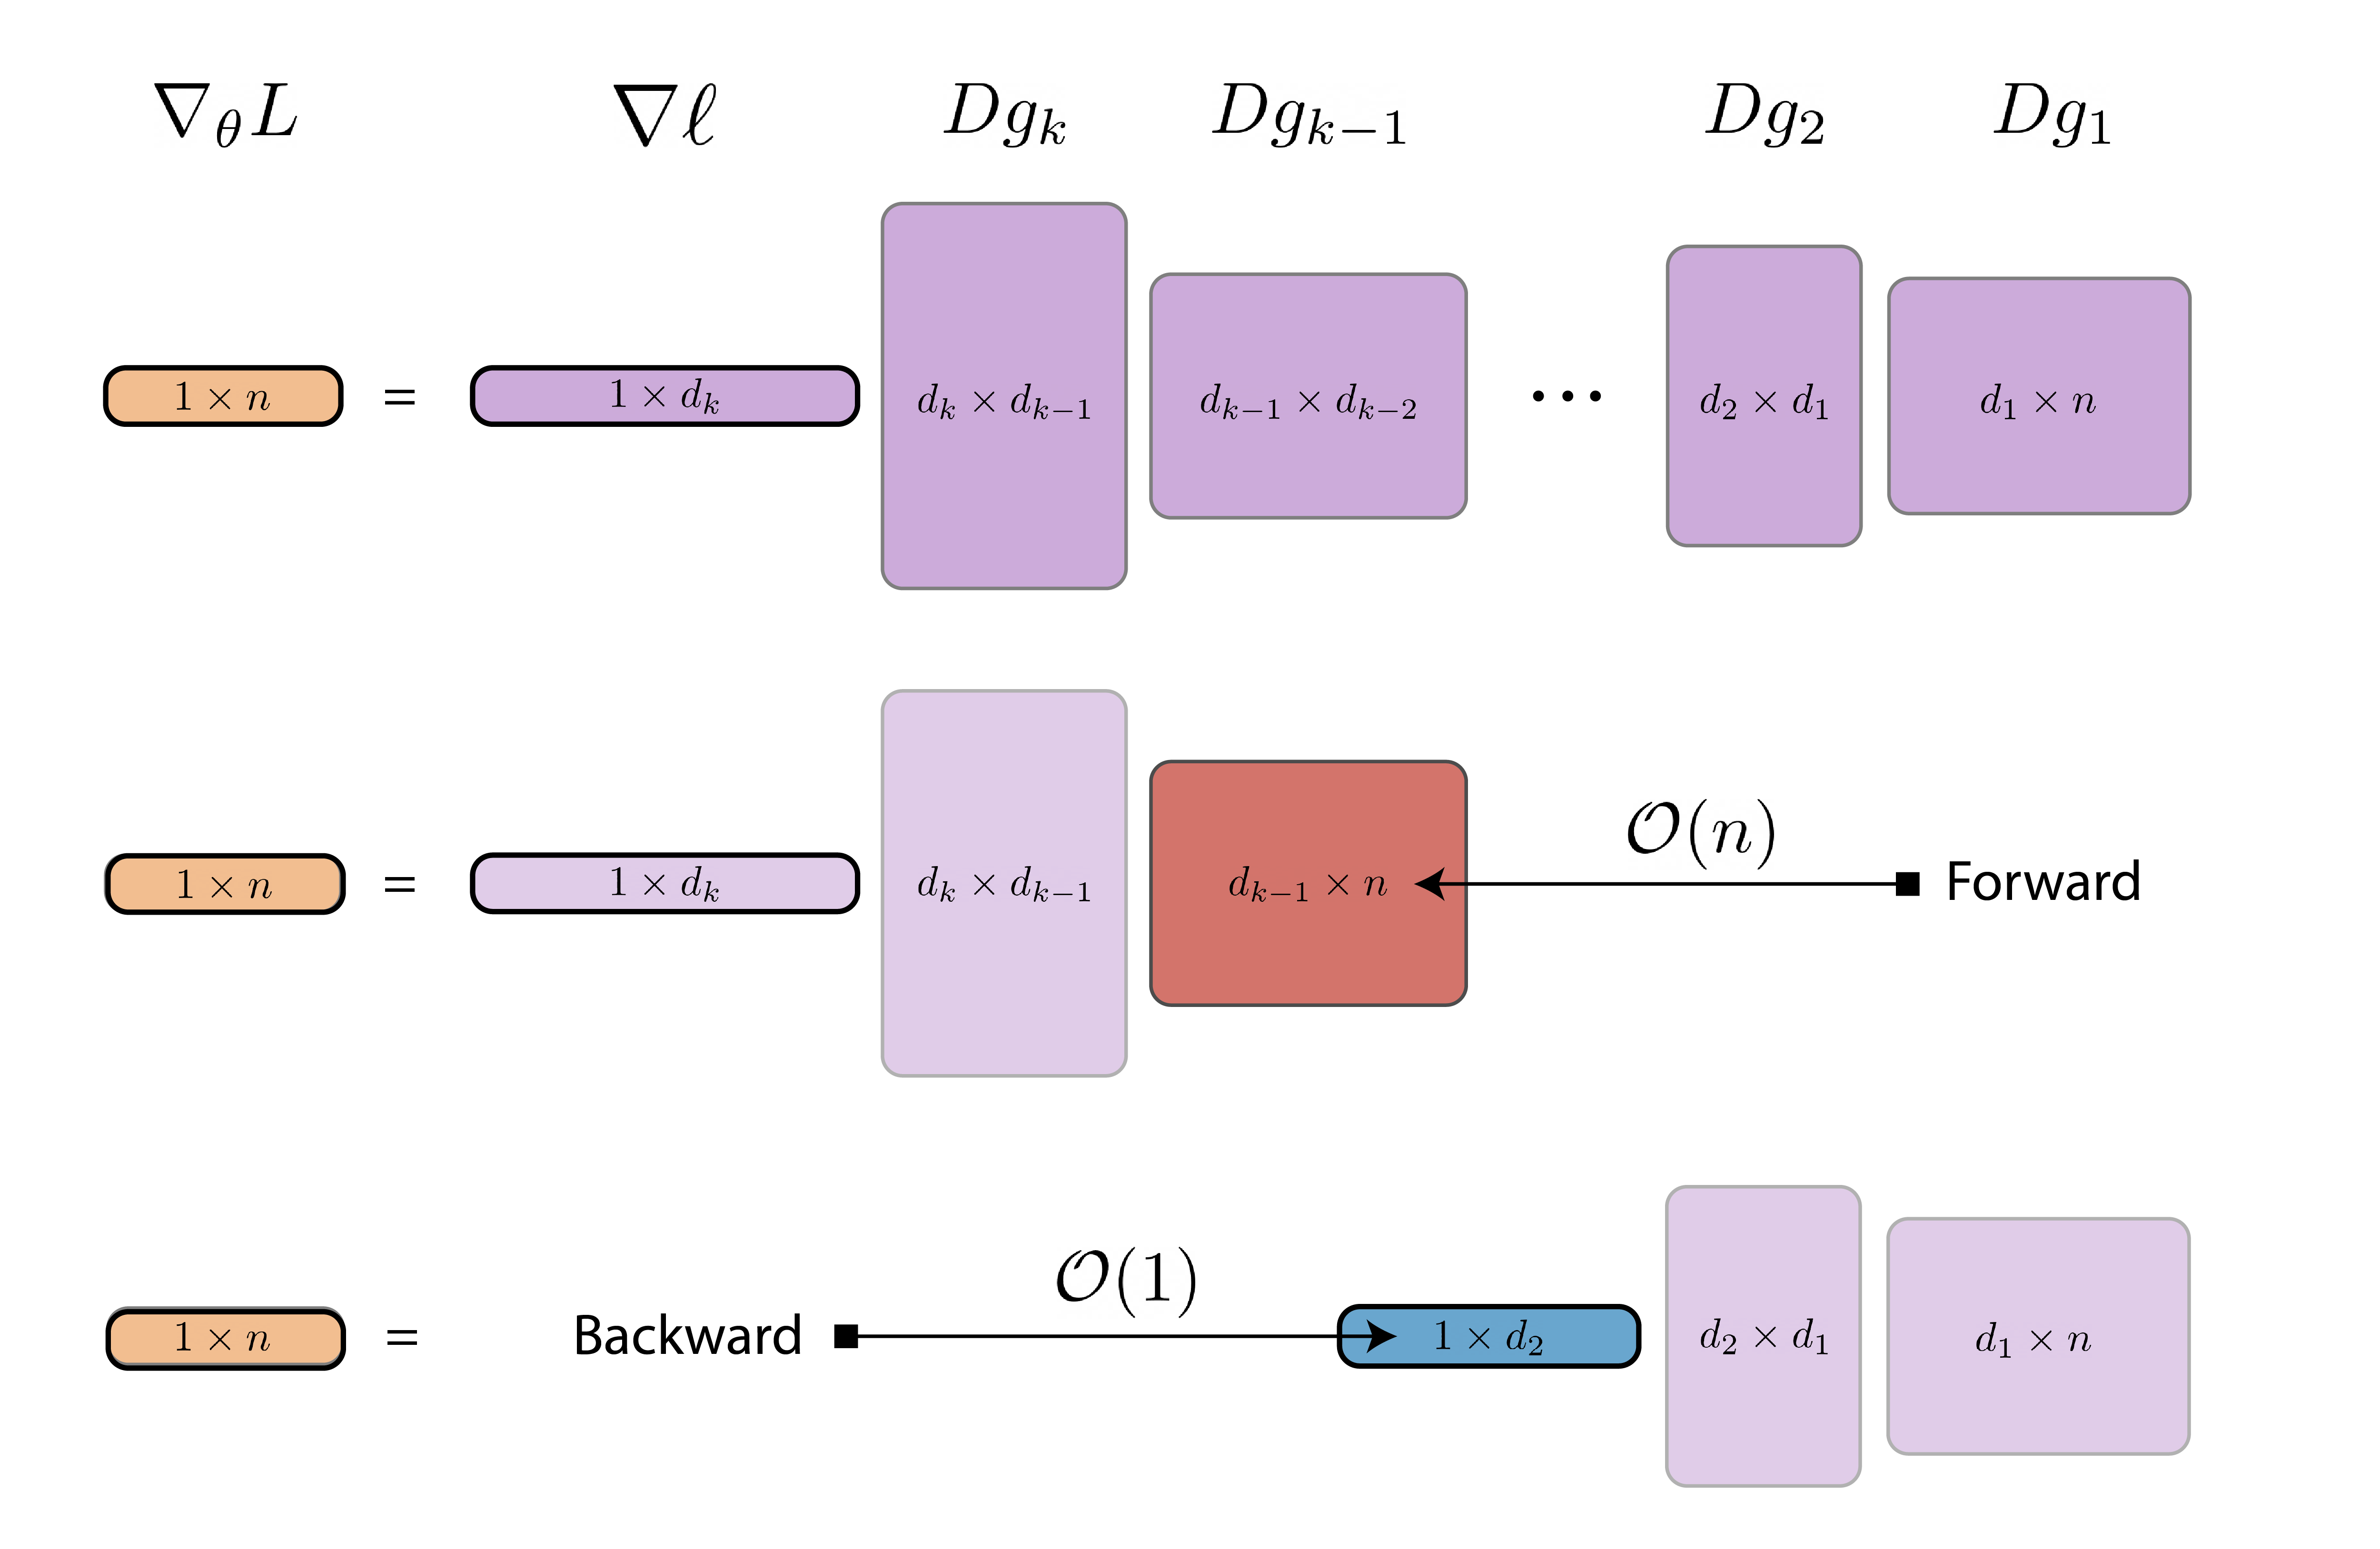
\includegraphics[width=0.95\textwidth]{figures/VJP-JVP.png}
    \caption{Comparison between forward and backward AD. Changing the order of how we multiply the Jacobians change the total number of floating-point operations, which leads to different computational complexities between forward and backward mode. However, backwards mode requires storing in memory information about the forward execution of the program, while forward mode can update the gradient on running time.}
    \label{fig:vjp-jvp}
\end{figure}
